\section{An example: The divergence point}
This example shows a simple \emph{toy model} for some cognitive process that is able to produce a
so called \emph{divergence point} \cite[e.g.,][]{Reingold2012}. A divergence point of two response-latency
distributions is the earliest time point at which the two distributions differ. Obviously, 
there exists no divergence point, if the two distributions are analytic 
(e.g., the convolution of Gamma distributions, \cite{Gelooven1999}) and there is some controversy
whether a cognitive model exists that is formed by simple \emph{processing stages} which has a
divergence point \cite[e.g.,][]{Gomez2016}.

Within this example I not only show how a non-analytic response-latency distribution may arise
using very common processing-stage models (i.e., these stages are also used in EZ-Reader model,
\cite{Reichle2003}) that allows for a divergence point, but actually has a divergence point%
\footnote{At least one distribution being non-analytic is a necessary but not a sufficient
condition for the existence of a divergence point.}. 

This very simple model consists of 4 Gamma-distributed stages $V, S_1, S_2$ and $M$,
where the second stage $S_2$ is delayed by $500$ ms. 
The model is
\begin{align}
 \text{control: } & R_c = V + S_1 + M \\
 \text{experimental: } & R_e = V + \min(S_1, 500+S_2) + M\,,
\end{align}
where $V \sim \Gamma(5,30),\,S_1\sim\Gamma(10,50)\,S_2\sim\Gamma(1,200)$ and $M\sim\Gamma(1,150)$.
\begin{figure}[!ht]
 \centering
 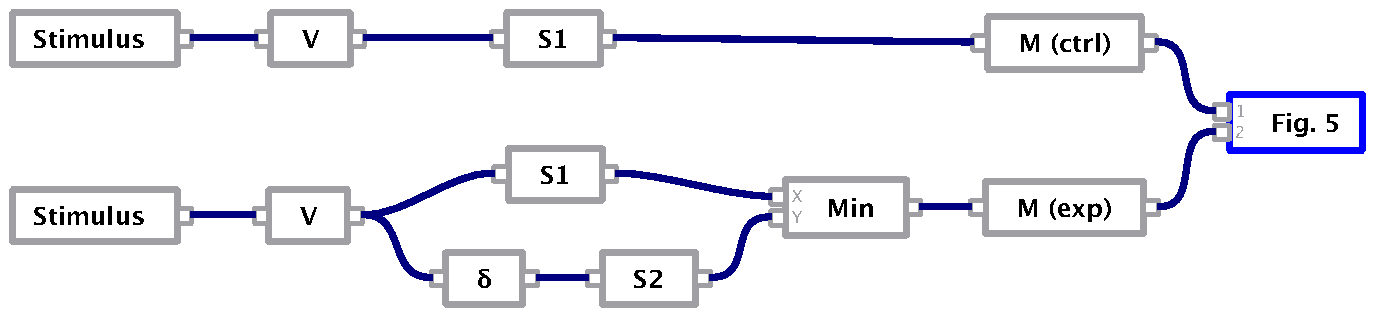
\includegraphics[width=0.9\textwidth]{fig/example2.pdf}
 \caption{Network of the second example model as visualized by \pkg{StochBB}.} \label{fig:example2}
\end{figure}

This model (also shown in Figure \ref{fig:example2}) can be read as: Under control condition, the
stimulus triggers a common \emph{visual} stage $V$ which then triggers a second stage $S_1$ that
itself immediately triggers the response stage $M$. Under experimental condition, again the
stimulus triggers the common stage $V$ which then triggers $S_1$. Additionally to the stage $S_1$,
$V$ also triggers the delayed stage $S_2$ in parallel to $S_1$. The response stage $M$ is then triggered by 
either $S_1$ or $S_2$, depending on which stage completes first. Consequently, the response latency
under experimental condition is $R_e = V + \min(S_1,S_2+500) + M$.

\begin{figure} [!ht]
 \begin{subfigure}[t]{0.45\textwidth}
   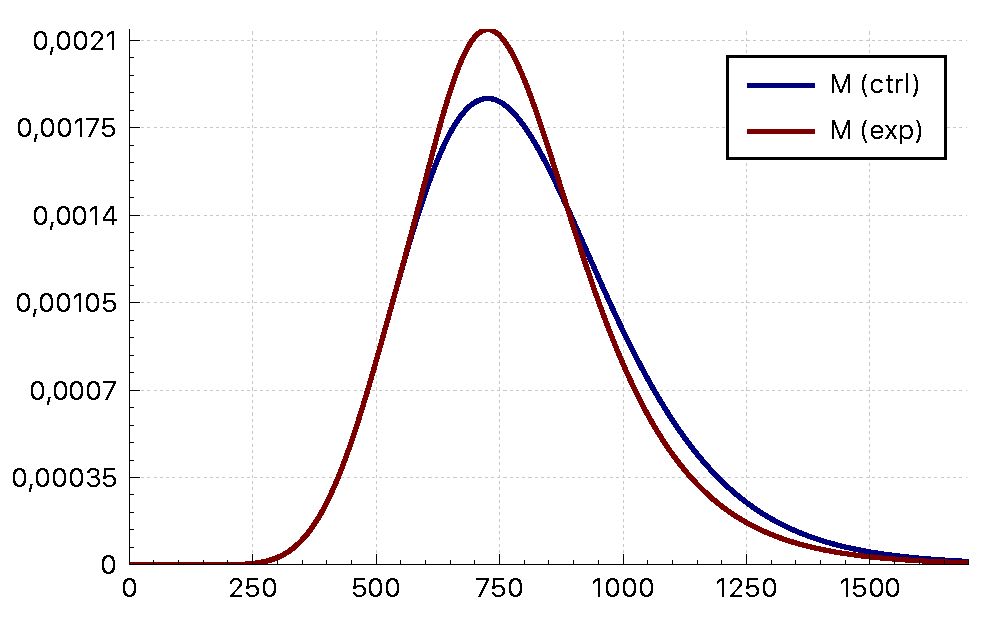
\includegraphics[width=.95\textwidth]{fig/example2_plot.pdf}
   \subcaption{PDFs of the response latencies under control condition (blue lines) and experimental condition (red lines).  
   The \emph{true} divergence point of the two response-latency distributions is $500$ ms, however, the distributions appear 
   to diverge much later (about $600$ ms). \label{fig:pod}}
  \end{subfigure} \hfill
 \begin{subfigure}[t]{0.45\textwidth}
   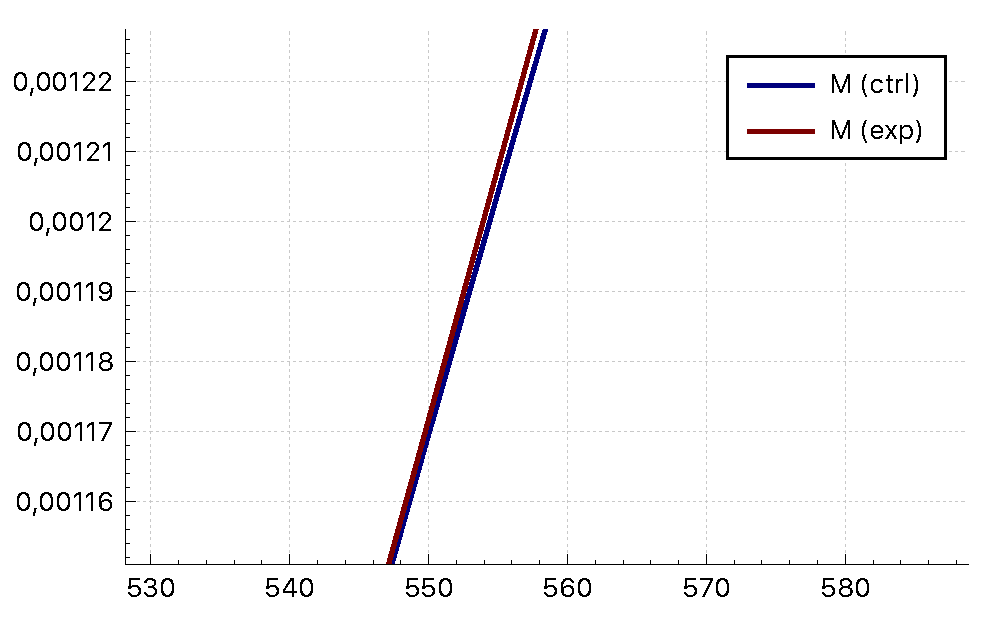
\includegraphics[width=.95\textwidth]{fig/example2_zoom_plot.pdf}
   \subcaption{The same PDFs but zoomed in. Here it get visible that the \emph{true} PD is much earlier that visible in the right plot. In fact the \emph{true} DP is not visible under any zoom level, as the PDFs diverge very slowly.} \label{fig:podzoom}
  \end{subfigure}
  \caption{Comparison of the response latency distributions as obtained from the mode shown in Fig. \ref{fig:example2}.}
  \label{fig:podplots}
\end{figure}

Figure \ref{fig:podplots} shows the plots generated by \pkg{StochBB}. The blue lines show the PDF
of the response latency under control condition. Being a convolution of 3 Gamma distributions, it 
is an analytic function on the interval $(0,\infty)$ \citep{Gelooven1999}. The red lines show the 
PDF of the response latency under experimental condition. As the distribution of $S_2$ is not analytic on 
the complete interval $(0,\infty)$ (discontinuity at $T=500$ ms), a divergence point may exist at 
$T=500$. 

Due to the \emph{minimum} stage and the fact that $P(S_2<500)=0$ (delayed by 
$500$ ms), it is ensured that the two response latencies are identical on the interval $[0,500)$ ms.
Hence, this simple model is able to produce a divergence point as both response-latency distributions are identical
on the interval $[0,500)$ and diverge thereafter.

However, Fig. \ref{fig:podzoom} shows that this divergence point cannot be estimated reliably from
a finite data set as the two response latency distributions diverge very slowly%
\footnote{In fact, the distribution of the response latency under experimental condition is an
example of a $C^\infty$-function, that is a smooth function, that is not analytic
($\notin C^\omega$).}. Consequently, an estimate for this point \cite[e.g. by means of estimators 
proposed in][]{Reingold2012} based on a finite sample will always be heavily biased towards larger
values. Moreover, if the experimental manipulation also affects the parameters of the $V, S1$ or 
$M$ stage, the two response distributions will be different everywhere on the interval
$(0,\infty)$ and consequently no divergence point exists. For a finite data set, however, an
estimator \cite[like][]{Reingold2012} will always report a finite estimate as it is simply impossible
to test for the existence of a divergence point on a finite data set. 